\documentclass{article}

\usepackage{fontspec}
\usepackage{tikz}

\title{Beikaitoru:\\an OpenType Hershey revival}
\author{Matthew Skala}

\defaultfontfeatures{Path=otf/}

\setsansfont{Beikaitoru506}
\setmainfont{Beikaitoru406}

\usetikzlibrary{calc}

\newcommand{\SegRad}{0.79}
\newcommand{\FatSegment}[2]{%
($(#1)!\SegRad cm!90:(#2)$) %
  ..controls ($(#1)!1.12*\SegRad cm!120:(#2)$) %
         and ($(#1)!1.12*\SegRad cm!150:(#2)$).. %
($(#1)!-\SegRad cm!0:(#2)$) %
  ..controls ($(#1)!1.12*\SegRad cm!-150:(#2)$) %
         and ($(#1)!1.12*\SegRad cm!-120:(#2)$).. %
($(#1)!\SegRad cm!-90:(#2)$) -- %
($(#2)!\SegRad cm!90:(#1)$) %
  ..controls ($(#2)!1.12*\SegRad cm!120:(#1)$) %
         and ($(#2)!1.12*\SegRad cm!150:(#1)$).. %
($(#2)!-\SegRad cm!0:(#1)$) %
  ..controls ($(#2)!1.12*\SegRad cm!-150:(#1)$) %
         and ($(#2)!1.12*\SegRad cm!-120:(#1)$).. %
($(#2)!\SegRad cm!-90:(#1)$) -- %
cycle %
}

\begin{document}
\maketitle

%%%%%%%%%%%%%%%%%%%%%%%%%%%%%%%%%%%%%%%%%%%%%%%%%%%%%%%%%%%%%%%%%%%%%%%%

Please note that this is a preliminary and incomplete version of the
Beikaitoru fonts and documentation.

\section{The Hershey fonts}

In 1967, Allen V.\ Hershey of the U.S.\ Naval Weapons Laboratory in
Dahlgren, Virginia published a set of fonts for use with computer-controlled
plotters.  At that time, very few digital fonts were available at all, and
even fewer were freely usable.  The Hershey fonts, being public domain
because of their origin as work produced by a U.S.\ Federal Government
employee in the course of his duties, quickly because popular.  They were
eventually distributed by the U.S.\ National Bureau of Standards (which is
sometimes incorrectly credited as the origin of the fonts), then
disseminated on Usenet and in many other ways.

The plotters for which the Hershey fonts were originally designed are now
long since obsolete.  The distinctive appearance of these fonts, which
results from the constraints of those plotters, is quite different from the
look of modern digital typography.  But because the Hershey fonts were (and
to some extent still are) so widely used, they have a nostalgic familiarity
for many present-day computer users.  They evoke early CAD systems,
low-budget GIS, and Turbo Pascal BGI drivers.  This package is a present-day
(2010s) revival of the Hershey fonts with current technology, based as
nearly as possible on the original source material and including many
special features omitted from other versions.

Beikaitoru is a parasite package of the Tsukurimashou project, whose home
page is at http://tsukurimashou.sourceforge.jp/.  Distribution packages of
Tsukurimashou include current development versions of Beikaitoru, but
Beikaitoru also has release packages of its own which may be more stable. 
Like Tsukurimashou, Beikaitoru (as a package, which includes significant
amounts of 21st-Century software by Matthew Skala beyond Hershey's
public-domain vector data) is distributed under the GNU General Public
License version 3 (included in the COPYING file), with the following
addition:

\begin{quotation}
As a special exception, if you create a document which uses this font, and
embed this font or unaltered portions of this font into the document, this
font does not by itself cause the resulting document to be covered by the
GNU General Public License. This exception does not however invalidate any
other reasons why the document might be covered by the GNU General Public
License. If you modify this font, you may extend this exception to your
version of the font, but you are not obligated to do so. If you do not wish
to do so, delete this exception statement from your version.
\end{quotation}

%%%%%%%%%%%%%%%%%%%%%%%%%%%%%%%%%%%%%%%%%%%%%%%%%%%%%%%%%%%%%%%%%%%%%%%%

\section{CRT plotters}

In order to understand the peculiarities of Hershey's fonts, it is
necessary to understand the technological environment in which he was
working.  The Naval Weapons Laboratory had a couple of Stromberg-Carlson
SC~4010 dot plotters, which operated by firing a beam of electrons onto a
phosphor-coated screen.  The resulting image would be recorded on
photographic film.  The beam passed through an aperture plate with a
selection of different holes that could shape it to look like different text
characters; then it was directed to a controllable location on the screen. 
So as long as you were content with the font built into the aperture plate,
you could plot characters easily and they would be high-resolution.  But
there was only one font consisting of 64 glyphs at one fixed size, and it
was sealed inside a big expensive vacuum tube.

If you wanted to plot anything else, you would have to use the machine in
"dot plotter" mode, by selecting a generic small round hole in the aperture
plate and then stamping the resulting circular dots at appropriate
coordinates to build up the image.  This was not a pixel-based system as we
usually imagine them, because the dots were always round and were a fair bit
larger than the accuracy to which they could be positioned; so the distance
between two lines might be adjustable in increments about a third the
smallest width of a line.  Because the dots were round, with careful
programming it was possible to smooth out most of the jaggies that would
otherwise appear in a grid-based image.  The dots were also fuzzy, with more
electrons near the centre than near the edges, and that also provided a
certain amount of built-in antialiasing.

Hershey's original report contained a set of fonts designed for the dot
plotters:  lists of coordinates at which to place dots so that they would
overlap to form glyphs.  Again, these are not the same thing as
pixel-based bitmap fonts, because the dot locations are expressed to finer
resolution than the sizes of the dots.  One thing that made it a non-trivial
exercise was that the time needed to plot each dot was significant when
multiplied by the number of dots per character and the number of characters
per page; so it was important to minimize the number of dots used while
making the characters look as good as possible.  The Hershey dot fonts,
although interesting, never became popular and are not included in this
version of Beikaitoru.  (Maybe in a future version...)

The next step up in technology was the SC~4020.  It's not clear to me from
his initial report whether Hershey actually had access to one these in 1967,
or just its specifications and output samples, but the fact that he created
a suite of fonts suitable for devices like it makes me think he must have
had access to some device at least sort of like the SC~4020.  It worked on
the same basic principle as the SC~4010, but it could also sweep the
electron beam smoothly from one grid point to another.  Images formed in
this vector-plotting mode would consist of fattened line segments (the set
of all points within a certain fixed radius of any point on any of a set of
line segments) where the endpoints were all on an integer grid, the spot
diameter was bigger than the grid size, and the segments, despite having
their endpoints snapped to the grid, were smooth to a much higher precision
than the grid itself.  Despite there being a grid involved, there still were
no pixels.

Hershey also wrote about an SC~4060, which was basically the same technology
as the SC~4020 but enhanced to run at higher speed and with a wider range of
ready-made glyphs built into its aperture plate; and a "Linotron" printer,
(not clear whether it is related to the well-known Linotronic
phototypesetting machines) which operated like the SC~4020 in vector mode
but instead of the aperture plate had an optical scanner that functioned as
a read-only memory to provide raster-scanned character definitions that the
host computer could invoke at different scales.  Presumably the film in the
Linotron's optical scanner could be swapped out to provide a selection of
fonts.

The Hershey fonts that everybody remembers are the ones he suggested for use
with the SC~4060.  They consist of lists of line segments with the endpoints
on grid points.  The grid is quite coarse relative to the size of the
letters.  Hershey's guideline was 21 grid units for the height of capital
letters in large sizes; so the grid size might be thought of as comparable
to present-day screen bitmap grids.  But these vectors are neither bitmaps,
nor outlines like those in a modern "vector" font; instead they are paths
along which it is assumed the machine will sweep a circular pen.  The pen
size is only vaguely specified, but assumed to be bigger than the grid.

%%%%%%%%%%%%%%%%%%%%%%%%%%%%%%%%%%%%%%%%%%%%%%%%%%%%%%%%%%%%%%%%%%%%%%%%

\section{Pen size}

Figure~\ref{fig:capa-normal} shows a typical glyph ("occidental glyph 3001,
triplex Roman capital A") from the Hershey vector collection.  The pen size
shown is 1.59 times the grid spacing.  This seems to be close to how Hershey
intended the glyph should appear, when he originally designed it.  The wide
stroke along the side is made from three segments that overlap to form a
solidly filled wide stroke, and there are no gaps inside the filled outline
of the glyph.

\begin{figure}
  \centering\renewcommand{\SegRad}{0.79}
  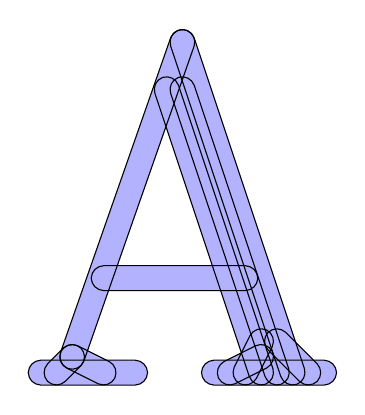
\begin{tikzpicture}[scale=0.2]
    \fill[color=blue!30!white] \FatSegment{0,12}{-7,-8};
    \fill[color=blue!30!white] \FatSegment{-1,9}{5,-9};
    \fill[color=blue!30!white] \FatSegment{0,9}{6,-9};
    \fill[color=blue!30!white] \FatSegment{0,12}{7,-9};
    \fill[color=blue!30!white] \FatSegment{-5,-3}{4,-3};
    \fill[color=blue!30!white] \FatSegment{-9,-9}{-3,-9};
    \fill[color=blue!30!white] \FatSegment{2,-9}{9,-9};
    \fill[color=blue!30!white] \FatSegment{-7,-8}{-8,-9};
    \fill[color=blue!30!white] \FatSegment{-7,-8}{-5,-9};
    \fill[color=blue!30!white] \FatSegment{5,-8}{3,-9};
    \fill[color=blue!30!white] \FatSegment{5,-7}{4,-9};
    \fill[color=blue!30!white] \FatSegment{6,-7}{8,-9};
    \draw \FatSegment{0,12}{-7,-8};
    \draw \FatSegment{-1,9}{5,-9};
    \draw \FatSegment{0,9}{6,-9};
    \draw \FatSegment{0,12}{7,-9};
    \draw \FatSegment{-5,-3}{4,-3};
    \draw \FatSegment{-9,-9}{-3,-9};
    \draw \FatSegment{2,-9}{9,-9};
    \draw \FatSegment{-7,-8}{-8,-9};
    \draw \FatSegment{-7,-8}{-5,-9};
    \draw \FatSegment{5,-8}{3,-9};
    \draw \FatSegment{5,-7}{4,-9};
    \draw \FatSegment{6,-7}{8,-9};
  \end{tikzpicture}
  \caption{A typical glyph drawn with pen size 1.59 grid units.}
  \label{fig:capa-normal}
\end{figure}

Consider Figure~\ref{fig:capa-thin}, which shows a magnified view of the top
of the same glyph, drawn with a pen size of 1.26 grid units.  There is a
small, roughly triangular area uncovered inside the corner, where the
central filling stroke doesn't extend quite far enough to fill the entire
space formed by the other strokes.  The smaller the pen size, the more of
these defects occur.  However, on an actual CRT plotter, the dots don't have
sharp edges; instead of having a stark white defect in the middle of the
corner, the actual CRT plotter would produce a soft-edged light grey area
where the edges of the filling stroke partially filled in the gap.  Some of
that effect is visible in copies of Allen V.\ Hershey's original technical
report; it appears that he printed it using some kind of machine with a dot
size of somewhere around 1.2, but fuzzy edges that made these gaps less
visible.

\begin{figure}
  \centering\renewcommand{\SegRad}{0.63}
  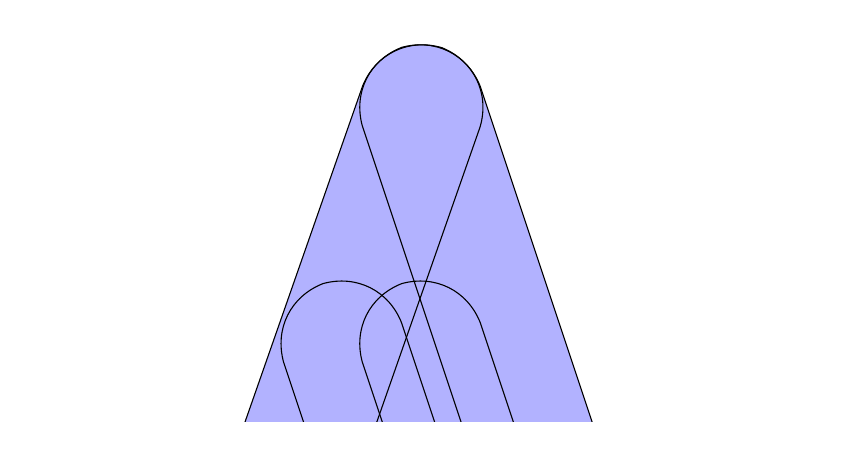
\begin{tikzpicture}[scale=1]
    \path[clip] (-5,8) rectangle (5,13);
    \fill[color=blue!30!white] \FatSegment{0,12}{-7,-8};
    \fill[color=blue!30!white] \FatSegment{-1,9}{5,-9};
    \fill[color=blue!30!white] \FatSegment{0,9}{6,-9};
    \fill[color=blue!30!white] \FatSegment{0,12}{7,-9};
    \draw \FatSegment{0,12}{-7,-8};
    \draw \FatSegment{-1,9}{5,-9};
    \draw \FatSegment{0,9}{6,-9};
    \draw \FatSegment{0,12}{7,-9};
  \end{tikzpicture}
  \caption{Detail drawn with pen size 1.26 grid units.}
  \label{fig:capa-thin}
\end{figure}

For a modern vector font, meant for output devices with much less fuzziness,
it is not clear how to proceed.  Filling in all the gaps requires using a
pen size well over 1.6; but that will have the effect of filling in some
gaps (particularly in the more detailed Japanese kanji glyphs) that were
obviously intended not to be filled.  Reducing the pen width enough to keep
everything separated that should be, will inevitably introduce some unfilled
gaps.  There is no pen size that completely avoids both issues.  Beikaitoru
provides a selection of several different weights corresponding to different
pen sizes, but short of modifying the vectors to add extra gap-filling
strokes, no perfect solution is possible.

Many historical users of the Hershey fonts used much smaller pen sizes than
these anyway.  The Naval Weapons Lab's CRT plotters had limited resolution
and needed to plot glyphs only a few grid cells high.  Scaling the fonts was
not practical because of integer rounding concerns, anticipating the
"hinting" issues in vector fonts designed much later for use on pixel-based
displays.  In order to have different sizes of lettering, Hershey designed
complete new sets of vectors for each different size; each set would only be
used at its fixed native size.  But just a few years later, when the CAD/CAM
and GIS communities were using the Hershey fonts with pen plotters and
high-resolution vector CRTs, they had equipment capable of scaling the
fonts, and that's what they did.

It was common practice to scale the Hershey vectors to an arbitrary variable
size while not scaling the pen at all.  The pen size would usually end up
much smaller than the grid size.  This scaling would deliberately expose the
structure of the filling-in strokes that were originally meant to be hidden
by overlap.  Figure~\ref{fig:capa-vthin} shows the result.  This visual
style, much different from what appears in the original Hershey report, is
the style that many people today remember as the classic style of the
Hershey fonts.

\begin{figure}
  \centering\renewcommand{\SegRad}{0.125}
  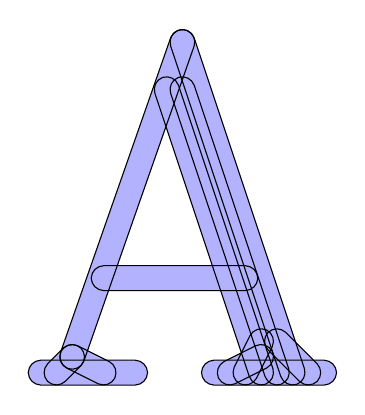
\begin{tikzpicture}[scale=0.2]
    \fill[color=blue!30!white] \FatSegment{0,12}{-7,-8};
    \fill[color=blue!30!white] \FatSegment{-1,9}{5,-9};
    \fill[color=blue!30!white] \FatSegment{0,9}{6,-9};
    \fill[color=blue!30!white] \FatSegment{0,12}{7,-9};
    \fill[color=blue!30!white] \FatSegment{-5,-3}{4,-3};
    \fill[color=blue!30!white] \FatSegment{-9,-9}{-3,-9};
    \fill[color=blue!30!white] \FatSegment{2,-9}{9,-9};
    \fill[color=blue!30!white] \FatSegment{-7,-8}{-8,-9};
    \fill[color=blue!30!white] \FatSegment{-7,-8}{-5,-9};
    \fill[color=blue!30!white] \FatSegment{5,-8}{3,-9};
    \fill[color=blue!30!white] \FatSegment{5,-7}{4,-9};
    \fill[color=blue!30!white] \FatSegment{6,-7}{8,-9};
    \draw \FatSegment{0,12}{-7,-8};
    \draw \FatSegment{-1,9}{5,-9};
    \draw \FatSegment{0,9}{6,-9};
    \draw \FatSegment{0,12}{7,-9};
    \draw \FatSegment{-5,-3}{4,-3};
    \draw \FatSegment{-9,-9}{-3,-9};
    \draw \FatSegment{2,-9}{9,-9};
    \draw \FatSegment{-7,-8}{-8,-9};
    \draw \FatSegment{-7,-8}{-5,-9};
    \draw \FatSegment{5,-8}{3,-9};
    \draw \FatSegment{5,-7}{4,-9};
    \draw \FatSegment{6,-7}{8,-9};
  \end{tikzpicture}
  \caption{Glyph drawn with pen size 0.25 grid units.}
  \label{fig:capa-vthin}
\end{figure}

To summarize:  Hershey's report quotes dot sizes of 2.9 grid units for the
SC~4010 printer (not strictly comparable to the others because it was not a
vector printer); 2.3 for the SC~4020; and "could be as small as" 1.0 for the
SC~4060.  He also implied that smaller was better, down to the minimum of
1.0 needed to allow dots to overlap at all, which seemed not to be
achievable with 1967 technology.  It appears that Hershey's vector designs
were in fact intended for plotting with the equivalent of a sharp-edged dot
of about 1.6 grid units diameter; but in practice he would have achieved
that with a somewhat smaller fuzzy-edged dot instead.  The examples in his
report seem to have been plotted with a fuzzy dot size near 1.2, which may
have been slightly smaller than ideal.  And then subsequent to Hershey's
work, many users ended up choosing much smaller dot sizes, producing a very
different look.

Beikaitoru provides the following nine numbered sizes:

\begin{tabular}{ll}
  size & dot diameter \\ \hline
  1 & 0.125 \\
  2 & 0.250 \\
  3 & 0.500 \\
  4 & 1.000 \\
  5 & 1.260 \\
  6 & 1.587 \\
  7 & 2.000 \\
  8 & 2.520 \\
  9 & 3.175
\end{tabular}

Size 6 is probably optimal for simulating the way Hershey intended his fonts
to look on the hardware that was current in 1967, and it is the size used to
typeset the main text of this documentation.  Sizes 1, 2, and 3, depending
on scaling, may be appropriate for simulating later historical uses of the
Hershey vectors in vector-plotting environments.

\end{document}
